\documentclass[11pt]{article}
% Switch [review] to [preprint] for a non-anonymous arXiv version, [final] for camera-ready.
\usepackage[review]{acl}
\usepackage{times}
\usepackage{latexsym}
\usepackage[T1]{fontenc}
\usepackage[utf8]{inputenc}
\usepackage{microtype}
\IfFileExists{inconsolata.sty}{\usepackage{inconsolata}}{}
\usepackage{graphicx}
% Shared macros. Placeholders are red so nothing slips into a submission.
\usepackage{xcolor}
\usepackage{booktabs,multirow,array,amsmath,amssymb,url}
\usepackage{pgfplots}
\usepackage{tikz}
\usepgfplotslibrary{groupplots}
\pgfplotsset{compat=1.17}
\usetikzlibrary{patterns,arrows.meta,positioning,shapes.geometric,fit,calc}

\newcommand{\xx}{\textcolor{red}{\textbf{XX}}}            % numeric placeholder
\newcommand{\todo}[1]{\textcolor{blue}{[TODO: #1]}}        % instruction to the runner
\newcommand{\phfig}{\node[rotate=22,gray!70,font=\large\bfseries] at (rel axis cs:0.5,0.5) {PLACEHOLDER};}
\newcommand{\bluff}{\textsc{BLUFF}}

% Colour-blind-safe palette for placeholder plots
\definecolor{cA}{HTML}{1B6CA8}
\definecolor{cB}{HTML}{D55E00}
\definecolor{cC}{HTML}{009E73}
\definecolor{cD}{HTML}{6C6C6C}


\title{Closing Language Disparities with LLM-Driven Weight Surgery:\\
Evidence from 58 Long-Tail Languages in \bluff}

\author{Jason S. Lucas \\
  Secure and Ethical AI Lab (SEAL), Department of Information Science \\
  University of Colorado Boulder \\
  \texttt{jason.lucas@colorado.edu} \\\And
  Collaborator XX \\
  Affiliation XX}

\begin{document}
\maketitle

\begin{abstract}
Multilingual detectors fine-tuned on mixed or high-resource data still leave long-tail languages behind: \bluff{} reports up to 25.3\% F1 degradation on low-resource languages relative to high-resource ones. The usual repairs (more fine-tuning, adapters, merging, neuron interventions) need a training run per language group and can erode what the model already does well. We ask whether a general LLM that reads and writes a model's weights as text, with no gradients, can close this gap more cheaply and with less collateral damage. We test this on \bluff{}, which covers 78 languages (20 big-head, 58 long-tail) and four detection tasks, after multilingual and cross-lingual fine-tuning. Surgery cuts the big-head versus long-tail F1 gap from \xx{} to \xx{} points, matches or beats adapters, merging and neuron baselines at \xx{}\% of their compute, and changes big-head F1 by \xx{} points. Gains concentrate in languages where a probe finds the signal in the representation but the classifier head misses it (an \emph{obstacle}), and vanish where the signal is absent (a \emph{missing capability}). We release the audit protocol and aggregate results, not edited weights.
\end{abstract}

\section{Introduction}
Language technology is uneven across languages. \bluff{} makes this concrete for false and synthetic content detection: across 78 languages, 20 of them big-head and 58 long-tail, detectors lose up to 25.3\% F1 on the long tail \citep{lucas2026bluff}. The same pattern appears for English dialects \citep{lucas2026diaharm}. The causes are well studied: capacity dilution in multilingual training \citep{conneau2020xlmr,chang2024curse}, tokenizer disparity \citep{petrov2023tokenizers}, and thin data for rare knowledge \citep{kandpal2023longtail}.

Repairs exist, but each has a price. Per-language adapters \citep{pfeiffer2020madx} and extra low-rank fine-tuning \citep{biderman2024lora} need training runs and labeled data per language. Merging \citep{ilharco2023task,tao2024merging} needs compatible checkpoints. Language-neuron interventions \citep{tang2024lape,gurgurov2025arithmetics} are cheap but may not transfer \citep{mondal2025neurons}. Knowledge editors \citep{meng2022rome,meng2023memit} target facts, and repeated edits can collapse general ability \citep{zhang2026revive}.

A new option appeared recently. \citet{takehi2026weightspace} report that a general LLM can read a small model's weights as text, propose edits, and apply them with only forward passes as feedback. On Qwen3.5-0.8B, removing one looping direction (0.016\% of weights, 50 forward passes) raised MATH-500 from 7.9\% to 48.1\%. On Gemma 3 270M the same approach gave no gain, which the authors read as edits removing obstacles but not adding missing ability. The evidence is a single blog post at up to 0.8B parameters, so it needs independent tests.

\paragraph{This paper.} We test whether weight surgery closes the language gap on \bluff{}, and where it cannot. Our contributions:
\begin{enumerate}\itemsep0pt
\item A protocol for language-targeted surgery of fine-tuned detectors that uses only $k$ validation examples per language, a fixed forward-pass budget, a regression guard, and a full audit log.
\item An obstacle-versus-missing-capability diagnostic based on the gap between a linear probe and the model's own head, used to predict which languages surgery can help.
\item An evaluation over 78 languages, two fine-tuning settings, seven baselines, and cost, regression, and autonomy ablations (Sections~\ref{sec:setup}--\ref{sec:results}).
\end{enumerate}

\section{Background and Related Work}
\paragraph{Long-tail effects in multilingual models.} Adding languages helps in moderation and then hurts all languages at fixed capacity \citep{conneau2020xlmr,chang2024curse}. Tokenization makes the same text cost up to 15 times more tokens in some languages \citep{petrov2023tokenizers}, a disparity that weights alone cannot remove. We therefore treat tokenizer cost as a covariate, not a target.

\paragraph{Fixing languages in weight space.} Language-specific neurons \citep{tang2024lape} can be steered \citep{gurgurov2025arithmetics}, but steering works less well for low-resource languages, and neuron-targeted LoRA did not improve cross-lingual transfer in one study \citep{mondal2025neurons}. Training-free weight edits have been used for multilingual safety \citep{liang2026sparse}, and a very small shared set of neurons carries safety across languages \citep{zhang2026safetyneurons}. Hypernetworks generate adapters from prompts \citep{liang2025dnd}, but need training on a library of adapters.

\paragraph{LLMs that modify models.} Agents that run experiments on other networks exist for interpretability \citep{rottshaham2024maia}. Weight-space programming \citep{takehi2026weightspace} goes further by letting the LLM write the weights. We build on that idea for a multilingual classification setting and add controls it lacks.

\section{Problem and Hypotheses}
\label{sec:problem}
Let $f_\theta$ be a detector fine-tuned on \bluff{} under a given training setting. For language $\ell$ let $F_1(\ell;\theta)$ be its macro-F1, and let $\mathcal{H}$ and $\mathcal{T}$ be the 20 big-head and 58 long-tail languages. The disparity gap is
\begin{equation}
G(\theta) = \frac{1}{|\mathcal{H}|}\sum_{\ell\in\mathcal{H}} F_1(\ell;\theta) - \frac{1}{|\mathcal{T}|}\sum_{\ell\in\mathcal{T}} F_1(\ell;\theta).
\end{equation}
Surgery returns edited weights $\theta'$ that minimize $G$ subject to a regression constraint on the big-head languages:
\begin{equation}
\begin{split}
\min_{\theta'}\; & G(\theta') \\
\text{s.t.}\; & \bar F_1^{\mathcal{H}}(\theta) - \bar F_1^{\mathcal{H}}(\theta') \le \delta, \\
& \|\theta'-\theta\|_0 \le \epsilon\,|\theta|.
\end{split}
\end{equation}
We pre-register six hypotheses (thresholds fixed before any test-split run, \todo{fill dated file}):
\begin{description}\itemsep0pt
\item[H1] Surgery lowers $G$ by at least \xx{} F1 points relative to the unedited model.
\item[H2] Surgery matches or beats the best of adapters, merging, and neuron baselines on $G$ at lower compute.
\item[H3] Big-head F1 changes by at most $\delta=1$ point (regression constraint holds).
\item[H4] Gains are larger for languages with a high obstacle score (Section~\ref{sec:diag}) and absent for the 270M negative control.
\item[H5] An autonomous surgeon with a regression guard is within \xx{} points of an expert-in-the-loop surgeon while using fewer human hours.
\item[H6] Recovered models keep their gain on data the surgeon never saw: on each of four shifts (held-out languages, held-out generators, other datasets, dialect variants), surgery retains at least \xx{} of its \bluff{} test gain, within \xx{} of the best baseline.
\end{description}

\section{Method}
\label{sec:method}
\begin{figure*}[t]
\centering
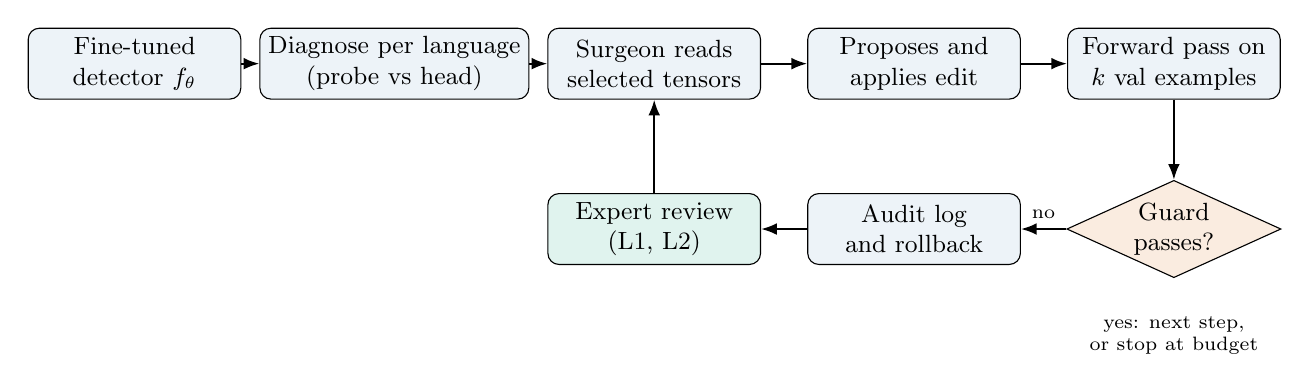
\begin{tikzpicture}[font=\small,
  box/.style={draw, rounded corners, align=center, minimum height=9mm, minimum width=2.7cm, inner sep=3pt, fill=cA!8},
  gate/.style={draw, diamond, aspect=2.2, align=center, inner sep=1pt, fill=cB!12},
  arr/.style={-{Latex[length=2mm]}, thick}]
\node[box] (ft) at (0,0) {Fine-tuned\\detector $f_\theta$};
\node[box] (diag) at (3.3,0) {Diagnose per language\\(probe vs head)};
\node[box] (read) at (6.6,0) {Surgeon reads\\selected tensors};
\node[box] (edit) at (9.9,0) {Proposes and\\applies edit};
\node[box] (fwd) at (13.2,0) {Forward pass on\\$k$ val examples};
\node[gate] (guard) at (13.2,-2.1) {Guard\\passes?};
\node[box] (log) at (9.9,-2.1) {Audit log\\and rollback};
\node[box, fill=cC!12] (human) at (6.6,-2.1) {Expert review\\(L1, L2)};
\node[font=\scriptsize, align=center] (yes) at (13.2,-3.45) {yes: next step,\\or stop at budget};
\draw[arr] (ft) -- (diag);
\draw[arr] (diag) -- (read);
\draw[arr] (read) -- (edit);
\draw[arr] (edit) -- (fwd);
\draw[arr] (fwd) -- (guard);
\draw[arr] (guard) -- node[above, font=\scriptsize]{no} (log);
\draw[arr] (log) -- (human);
\draw[arr] (human) -- (read);
\end{tikzpicture}
\caption{Surgery loop. The surgeon reads weights as text, edits, and receives only validation metrics. The regression guard can roll back any edit. At autonomy levels L1 and L2 a human reviews proposals; at L3 the human holds a veto. \todo{Replace with final vector figure.}}
\label{fig:method}
\end{figure*}

\subsection{Obstacle versus missing capability}
\label{sec:diag}
For each language $\ell$ we train a linear probe on frozen penultimate representations using the same $k$ examples the surgeon sees, and compare its macro-F1 with the model's own head:
\begin{equation}
o(\ell) = F_1^{\text{probe}}(\ell) - F_1^{\text{head}}(\ell).
\end{equation}
A large $o(\ell)$ means the representation carries the signal and something downstream blocks it: an \emph{obstacle}. A small or negative $o(\ell)$ with low probe F1 means the signal is not there: a \emph{missing capability}. Hypothesis H4 predicts surgery gain rises with $o(\ell)$.

\subsection{Surgery harness}
The surgeon is a general long-tool LLM with four tools: \texttt{read\_tensor(name, slice)}, \texttt{write\_tensor(name, patch)}, \texttt{forward(split)} returning F1 per language on validation data only, and \texttt{rollback(step)}. Tensors are serialized as text for the modules we expose (output projections and classifier layers of the last $L$ blocks; \xx{} parameters in total). Four knobs are fixed per run: forward-pass budget $B\in\{0,10,25,50\}$, edit budget $\epsilon\in\{0.01,0.1,1\}\%$ of weights, visible modules, and autonomy level (Section~\ref{sec:setup}).

\subsection{Regression guard and audit}
After each edit the guard (i) re-evaluates big-head validation F1 and rolls back if it falls by more than $\delta$, and (ii) checks that the leading singular directions of each edited matrix move less than a tolerance $\tau$, following the finding that general ability lives in the dominant spectrum \citep{zhang2026revive}. Every proposal, edit, metric, and rollback is logged to an append-only file.

\section{Experimental Setup}
\label{sec:setup}
\paragraph{Data.} \bluff{} (Table~\ref{tab:data}). The surgeon and all baselines see only $k\in\{16,64,256\}$ labeled validation examples per language. Test splits are held out and read once.

\begin{table}[t]
\centering\small
\begin{tabular}{lr}
\toprule
Item & Value \\
\midrule
Languages & 78 \\
\quad big-head / long-tail & 20 / 58 \\
Samples & 201K+ \\
\quad human / LLM-generated & 122K / $\sim$78K \\
mLLM generators & 19 \\
Tasks & 4 \\
Training settings & 6 \\
Settings used & multi., cross-ling. \\
\bottomrule
\end{tabular}
\caption{\bluff{} figures used in this paper (Hugging Face dataset card).}
\label{tab:data}
\end{table}

\paragraph{Models.} mDeBERTa-v3-base and XLM-R base detectors, plus multilingual S-BERT \citep{reimers2020making} and LaBSE \citep{feng2022labse} encoders (Hugging Face checkpoints \texttt{sentence-transformers/paraphrase-multilingual-mpnet-base-v2} and \texttt{sentence-transformers/LaBSE}) with a classification head, fine-tuned on \bluff{} under (a) the multilingual setting and (b) the cross-lingual setting (train on big-head, test on long-tail). Qwen3.5-0.8B and Gemma 3 270M serve as decoder tests and negative control. Surgeon identities: \xx{} (closed) and \xx{} (open weights).

\paragraph{Baselines.} B1 unedited; B2 extra LoRA on the same $k$ examples; B3 per-language adapters; B4 task-vector merging; B5 language-neuron intervention; B6 neuron-specific LoRA; B7 rank-one and batch editing (decoder models only).

\paragraph{Autonomy levels.} L0 human expert only; L1 surgeon proposes, human applies; L2 surgeon applies, human reviews each edit; L3 surgeon runs to budget, human holds a veto and reviews the audit log.

\paragraph{Out-of-distribution shifts (H6).} Edited models and baselines are frozen and then evaluated, without further edits, on four shifts that neither the surgeon nor any baseline sees: (i) held-out languages, where editing uses $k$ examples from half of a language group and testing uses the other half; (ii) held-out generators, meaning LLMs not among the 19 in \bluff{}; (iii) \xx{} external detection datasets; and (iv) dialect variants. The retention ratio is the F1 gain on the shifted set divided by the F1 gain on the \bluff{} test split. Shifted sets are chosen and listed before any test read.

\paragraph{Metrics and statistics.} Per-language macro-F1, $G$, worst-language F1, Gini of F1 across languages, and the share of long-tail languages within 5 points of the big-head mean. Regression: big-head F1 change plus one general NLU and one generation check (\xx{}). Cost: minutes, GPU-hours, surgeon tokens, dollars, percent of weights changed. Five seeds; bootstrap confidence intervals over languages; paired tests against B1 with Holm correction.

\section{Results}
\label{sec:results}
\todo{Replace every XX and every placeholder figure with outputs from runs/; keep the claim wording only if the result supports it.}

\paragraph{Main result (H1, H2).}
Table~\ref{tab:main} shows that surgery reduces $G$ from \xx{} to \xx{} points in the multilingual setting and from \xx{} to \xx{} in the cross-lingual setting. The best baseline reaches \xx{} and \xx{}. Figure~\ref{fig:gap} summarizes the gap by method.

\begin{table*}[t]
\centering\small
\begin{tabular}{l ccc ccc}
\toprule
& \multicolumn{3}{c}{Multilingual FT} & \multicolumn{3}{c}{Cross-lingual FT} \\
\cmidrule(lr){2-4}\cmidrule(lr){5-7}
Method & Big-head F1 & Long-tail F1 & Gap $G$ & Big-head F1 & Long-tail F1 & Gap $G$ \\
\midrule
B1 Unedited & \xx & \xx & \xx & \xx & \xx & \xx \\
B2 Extra LoRA & \xx & \xx & \xx & \xx & \xx & \xx \\
B3 Adapters & \xx & \xx & \xx & \xx & \xx & \xx \\
B4 Merging & \xx & \xx & \xx & \xx & \xx & \xx \\
B5 Neuron intervention & \xx & \xx & \xx & \xx & \xx & \xx \\
B6 Neuron-specific LoRA & \xx & \xx & \xx & \xx & \xx & \xx \\
\midrule
Surgery, L1 (expert applies) & \xx & \xx & \xx & \xx & \xx & \xx \\
Surgery, L3 (autonomous + guard) & \xx & \xx & \xx & \xx & \xx & \xx \\
\bottomrule
\end{tabular}
\caption{Main results on held-out \bluff{} test splits, mDeBERTa-v3-base, $k=64$, $B=50$, mean of five seeds. \todo{Add 95\% CIs in a second line or in the appendix. Repeat for XLM-R in the appendix.}}
\label{tab:main}
\end{table*}

\begin{figure}[t]
\centering
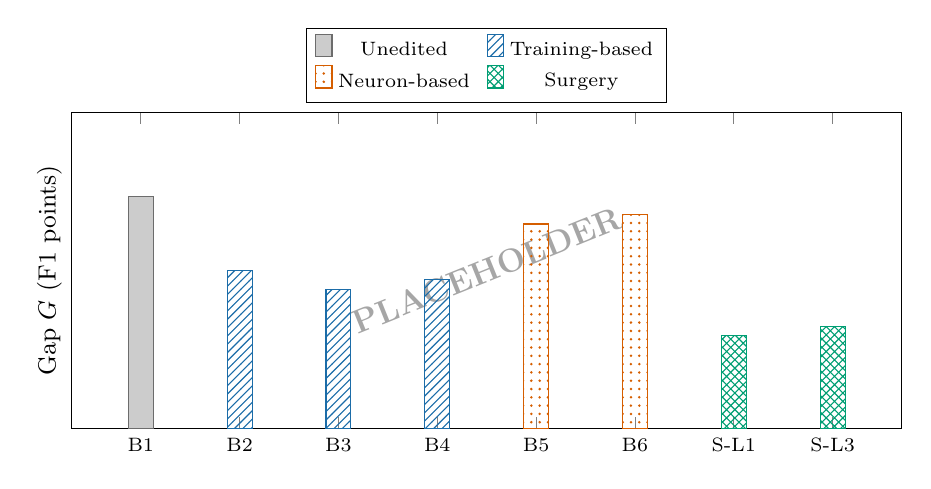
\begin{tikzpicture}
\begin{axis}[ybar stacked, width=\columnwidth, height=5.6cm, bar width=9pt,
  ylabel={Gap $G$ (F1 points)}, ymin=0, ymax=34, yticklabels={}, ytick=\empty,
  symbolic x coords={B1,B2,B3,B4,B5,B6,S-L1,S-L3}, xtick=data,
  x tick label style={font=\scriptsize}, ylabel style={font=\small},
  legend style={font=\scriptsize, at={(0.5,1.03)}, anchor=south, legend columns=2, /tikz/every even column/.append style={column sep=4pt}}]
\addplot[fill=cD!35, draw=cD] coordinates {(B1,25) (B2,0) (B3,0) (B4,0) (B5,0) (B6,0) (S-L1,0) (S-L3,0)};
\addplot[fill=white, draw=cA, pattern=north east lines, pattern color=cA] coordinates {(B1,0) (B2,17) (B3,15) (B4,16) (B5,0) (B6,0) (S-L1,0) (S-L3,0)};
\addplot[fill=white, draw=cB, pattern=dots, pattern color=cB] coordinates {(B1,0) (B2,0) (B3,0) (B4,0) (B5,22) (B6,23) (S-L1,0) (S-L3,0)};
\addplot[fill=white, draw=cC, pattern=crosshatch, pattern color=cC] coordinates {(B1,0) (B2,0) (B3,0) (B4,0) (B5,0) (B6,0) (S-L1,10) (S-L3,11)};
\legend{Unedited, Training-based, Neuron-based, Surgery}
\phfig
\end{axis}
\end{tikzpicture}
\caption{Placeholder: disparity gap by method (lower is better). The claim to test is that surgery (S-L1, S-L3) lowers $G$ at least as much as the best baseline. Bar heights are illustrative only. Patterns and colors mark method families: unedited (gray), training-based (blue, diagonal lines), neuron-based (orange, dots), surgery (green, crosshatch).}
\label{fig:gap}
\end{figure}

\paragraph{Compute and cost (H2).}
Table~\ref{tab:cost} reports cost. Surgery used \xx{} GPU-hours and \xx{} surgeon tokens per language group against \xx{} GPU-hours for adapters.

\begin{table}[t]
\centering\small
\begin{tabular}{l rrrr}
\toprule
Method & Min. & GPU-h & Tokens & \% wts \\
\midrule
B2 Extra LoRA & \xx & \xx & -- & \xx \\
B3 Adapters & \xx & \xx & -- & \xx \\
B4 Merging & \xx & \xx & -- & \xx \\
Surgery, L3 & \xx & \xx & \xx & \xx \\
\bottomrule
\end{tabular}
\caption{Cost per language group. Tokens are surgeon tokens. \% wts is percent of weights changed.}
\label{tab:cost}
\end{table}

\paragraph{Regression (H3).}
Table~\ref{tab:reg} shows big-head F1 changes by \xx{} points, within the $\pm1$ budget, and general NLU and generation checks change by \xx{} and \xx{}. Without the guard the same runs lose \xx{} big-head F1.

\begin{table}[t]
\centering\small
\begin{tabular}{l rrr}
\toprule
Condition & $\Delta$ big-head & $\Delta$ NLU & $\Delta$ NLG \\
\midrule
B2 Extra LoRA & \xx & \xx & \xx \\
B4 Merging & \xx & \xx & \xx \\
Surgery, guard on & \xx & \xx & \xx \\
Surgery, guard off & \xx & \xx & \xx \\
\bottomrule
\end{tabular}
\caption{Regression on languages and tasks the surgeon was not asked to change.}
\label{tab:reg}
\end{table}

\paragraph{Budget and the negative control (H4).}
Figure~\ref{fig:budget} shows $G$ falling with the forward-pass budget for the 0.8B decoder and staying flat for the 270M control. Edits beyond \xx{}\% of weights bring no further gain.

\begin{figure}[t]
\centering
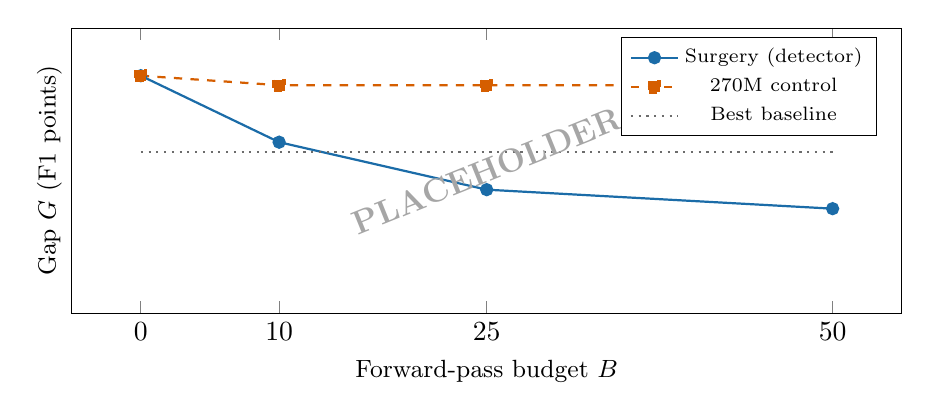
\begin{tikzpicture}
\begin{axis}[width=\columnwidth, height=5.2cm, xlabel={Forward-pass budget $B$}, ylabel={Gap $G$ (F1 points)},
  xtick={0,10,25,50}, ymin=0, ymax=30, yticklabels={}, ytick=\empty, legend style={font=\scriptsize, at={(0.97,0.97)}, anchor=north east},
  xlabel style={font=\small}, ylabel style={font=\small}]
\addplot[thick, cA, mark=*] coordinates {(0,25) (10,18) (25,13) (50,11)};
\addplot[thick, cB, dashed, mark=square*] coordinates {(0,25) (10,24) (25,24) (50,24)};
\addplot[thick, cD, dotted] coordinates {(0,17) (50,17)};
\legend{Surgery (detector), 270M control, Best baseline}
\phfig
\end{axis}
\end{tikzpicture}
\caption{Placeholder: gap versus forward-pass budget. The claim to test is a decline for detectors and no decline for the 270M control, which would support the obstacle reading.}
\label{fig:budget}
\end{figure}

\paragraph{Where it works (H4).}
Figure~\ref{fig:obstacle} plots per-language gain against obstacle score $o(\ell)$ for the 58 long-tail languages. The rank correlation is $\rho=\xx{}$ ($p=\xx{}$). Languages with $o(\ell)<\xx{}$ gain \xx{} points on average.

\begin{figure}[t]
\centering
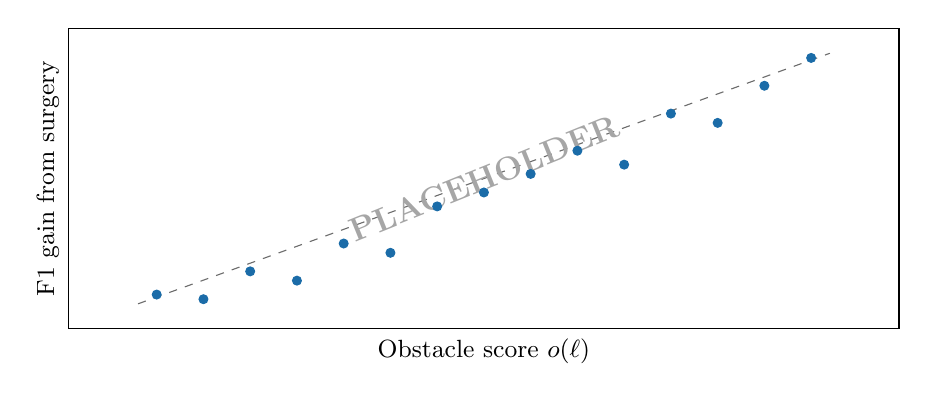
\begin{tikzpicture}
\begin{axis}[width=\columnwidth, height=5.4cm, xlabel={Obstacle score $o(\ell)$}, ylabel={F1 gain from surgery},
  xticklabels={}, xtick=\empty, yticklabels={}, ytick=\empty, xlabel style={font=\small}, ylabel style={font=\small}]
\addplot[only marks, mark=*, cA, mark size=1.6pt] coordinates {(0.5,0.3) (1,0.2) (1.5,0.8) (2,0.6) (2.5,1.4) (3,1.2) (3.5,2.2) (4,2.5) (4.5,2.9) (5,3.4) (5.5,3.1) (6,4.2) (6.5,4.0) (7,4.8) (7.5,5.4)};
\addplot[dashed, cD, no marks] coordinates {(0.3,0.1) (7.7,5.5)};
\phfig
\end{axis}
\end{tikzpicture}
\caption{Placeholder: per-language gain versus obstacle score. The claim to test is a positive relation: surgery helps when the signal is present but blocked, and not when it is missing.}
\label{fig:obstacle}
\end{figure}

\paragraph{By language family.}
Table~\ref{tab:family} breaks results down by family. Gains are largest for \xx{} and smallest for \xx{}, which also have the highest tokenizer cost ratio (\xx{}$\times$).

\begin{table}[t]
\centering\small
\begin{tabular}{l r rrr}
\toprule
Family & \#Lang. & $G$ before & $G$ after & Tok. ratio \\
\midrule
Family XX & \xx & \xx & \xx & \xx \\
Family XX & \xx & \xx & \xx & \xx \\
Family XX & \xx & \xx & \xx & \xx \\
Family XX & \xx & \xx & \xx & \xx \\
\bottomrule
\end{tabular}
\caption{Gap by language family. \todo{Use the family labels in the \bluff{} metadata.}}
\label{tab:family}
\end{table}

\paragraph{Autonomy (H5).}
Table~\ref{tab:autonomy} compares autonomy levels. L3 is within \xx{} points of L1 and needs \xx{} fewer expert hours.

\begin{table}[t]
\centering\small
\begin{tabular}{l rrrr}
\toprule
Level & $G$ & Expert h & Rollbacks & Bad edits \\
\midrule
L0 Human only & \xx & \xx & \xx & \xx \\
L1 Proposes & \xx & \xx & \xx & \xx \\
L2 Applies, reviewed & \xx & \xx & \xx & \xx \\
L3 Autonomous + veto & \xx & \xx & \xx & \xx \\
\bottomrule
\end{tabular}
\caption{Autonomy ablation. Bad edits are edits a native-speaker reviewer marks as harmful.}
\label{tab:autonomy}
\end{table}

\paragraph{Out-of-distribution transfer (H6).}
Table~\ref{tab:ood} and Figure~\ref{fig:ood} report retention on the four shifts. Surgery retains \xx{} of its \bluff{} gain on held-out languages and \xx{} on held-out generators, against \xx{} and \xx{} for the best baseline. Absolute gains over B1 are \xx{} to \xx{} points.

\begin{table}[t]
\centering\small
\setlength{\tabcolsep}{3.5pt}
\begin{tabular}{l rrrr}
\toprule
Method & Lang. & Gen. & Data & Dial. \\
\midrule
B2 LoRA & \xx & \xx & \xx & \xx \\
B3 Adapters & \xx & \xx & \xx & \xx \\
B4 Merging & \xx & \xx & \xx & \xx \\
B5 Neurons & \xx & \xx & \xx & \xx \\
B6 Neuron LoRA & \xx & \xx & \xx & \xx \\
Surgery (L3) & \xx & \xx & \xx & \xx \\
\bottomrule
\end{tabular}
\caption{Retention ratio (gain on shifted set divided by gain on the \bluff{} test split) by shift: held-out languages, generators, external datasets, dialect variants.}
\label{tab:ood}
\end{table}

\begin{figure}[t]
\centering
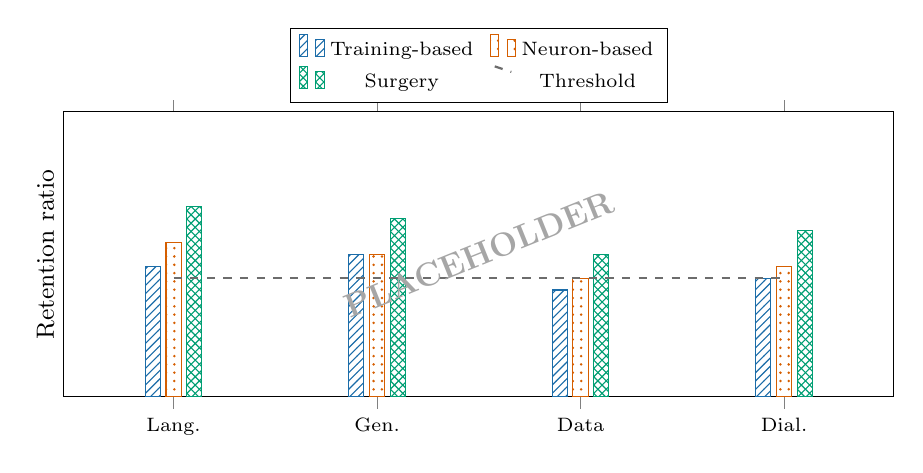
\begin{tikzpicture}
\begin{axis}[ybar, width=\columnwidth, height=5.2cm, bar width=5.5pt,
  ylabel={Retention ratio}, ymin=0, ymax=1.2, yticklabels={}, ytick=\empty,
  symbolic x coords={Lang.,Gen.,Data,Dial.}, xtick=data, enlarge x limits=0.18,
  x tick label style={font=\scriptsize}, ylabel style={font=\small},
  legend style={font=\scriptsize, at={(0.5,1.03)}, anchor=south, legend columns=2, /tikz/every even column/.append style={column sep=4pt}}]
\addplot[fill=white, draw=cA, pattern=north east lines, pattern color=cA] coordinates {(Lang.,0.55) (Gen.,0.60) (Data,0.45) (Dial.,0.50)};
\addplot[fill=white, draw=cB, pattern=dots, pattern color=cB] coordinates {(Lang.,0.65) (Gen.,0.60) (Data,0.50) (Dial.,0.55)};
\addplot[fill=white, draw=cC, pattern=crosshatch, pattern color=cC] coordinates {(Lang.,0.80) (Gen.,0.75) (Data,0.60) (Dial.,0.70)};
\addplot[thick, cD, dashed, sharp plot, mark=none] coordinates {(Lang.,0.5) (Dial.,0.5)};
\legend{Training-based, Neuron-based, Surgery, Threshold}
\phfig
\end{axis}
\end{tikzpicture}
\caption{Placeholder: retention ratio by shift type. The claim to test is that surgery stays above the threshold (dashed, \xx{}) and is no worse than the best baseline on every shift. Bar heights are illustrative only. Patterns and colors mark method families: training-based (blue, diagonal lines), neuron-based (orange, dots), surgery (green, crosshatch).}
\label{fig:ood}
\end{figure}

\section{Analysis}
\todo{Write after results. Planned analyses: (1) which modules were edited most; (2) five qualitative edit traces reviewed by native speakers; (3) failure cases where the surgeon overfit the $k$ examples (validation versus test gap); (4) sensitivity to $k$.}

\section{Discussion and Limitations}
Our evidence covers detectors up to \xx{} parameters and one primary benchmark. The method cannot repair tokenizer disparity or add knowledge that the model never learned, and a null result for languages with low obstacle scores would be expected. The surgeon sees $k$ labeled examples per language, which risks overfitting to the validation sample; we report the validation-to-test gap and the out-of-distribution retention in Table~\ref{tab:ood}, which tests only four shifts and models up to \xx{} parameters. Surgery is stochastic, so we report five seeds and the audit logs.

\section*{Ethics Statement}
Language-level edits can help communities with thin resources, but an autonomous editor can also be pointed at safeguards. A companion paper studies that risk in aggregate. We do not release edited weights or surgeon prompts that target safety behavior. Native-speaker reviewers were compensated at \xx{} per hour, and the review protocol was approved by \xx{}.

\section*{Acknowledgments}
\todo{Funding and compute (for example CU Boulder Alpine allocation), reviewers, and collaborators.}

\bibliography{references}

\appendix
\section{Reproducibility Checklist}
\begin{itemize}\itemsep0pt
\item Surgeon prompt template and tool schema: \todo{add after the harness is frozen}.
\item Hyperparameters: learning rates for B2 to B4, $\delta=1$, $\tau=\xx{}$, $k$, $B$, $\epsilon$.
\item Per-language results for all 78 languages: Table~\ref{tab:perlang} (\todo{generate from results.csv}).
\item Compute: GPU type, hours, and surgeon API cost.
\end{itemize}

\begin{table}[h]
\centering\small
\begin{tabular}{l rrr}
\toprule
Language & Before & After & Obstacle $o$ \\
\midrule
Lang.\ XX & \xx & \xx & \xx \\
\multicolumn{4}{c}{\ldots 78 rows}\\
\bottomrule
\end{tabular}
\caption{Per-language F1 before and after surgery (template).}
\label{tab:perlang}
\end{table}

\end{document}
